\documentclass{article}
\usepackage{graphicx}
\usepackage[fontsize=11pt]{scrextend}
\usepackage{float}
\title{PowerEnjoy Service - Project Plan}
\begin{document}

\begin{titlepage}
\begin{figure}
	\centering
	\includegraphics{polimi}
\end{figure}
\maketitle
\centering
Prof. Luca Mottola
\newline
\raggedleft
Authors:
\begin{itemize}
	\raggedleft
	\item ZHOU YINAN(Mat. 872686)
	\item ZHAO KAIXIN(Mat. 875464)
	\item ZHAN YUAN(Mat. 806508)	
\end{itemize}
\end{titlepage}

\tableofcontents
\newpage
\section{Introduction}
\subsection{Revision History}
Version 1.0
\subsection{Purpose and Scope}
This document aims at analyzing the overall complexity and making an estimation about the project size and required effort. The result will help project manager to decide the project budget, resource allocation and the schedule of activities.The document is divided into four parts. \\

In the first part of the document, We will use two specific methods to estimate the size and complexity of the project. First of all, we will use Function Points to calculate the average line of codes. Secondly, we will use COCOMO method to indicate the cost and effort estimation. \\

In the second part of the document, we will present the tasks for the project and the corresponding schedule. We will use the above results to come up with a suitable working plan covering the entire project development.\\

In the third part of the document, we will assign each team member specific missions to tickle down the project.\\

finally, we are going to analyze the risk we may encounter during the development. By analyzing the risk and coming up with possible solutions, we'll minimize the possibility for failure.
\subsection{Definitions, Acronyms, Abbreviations}
	\subsubsection{Definitions}
	\begin{itemize}
		\item Precedentedness: High if a product is similar to several previously developed projects
		\item Development Flexibility: High if there are no specific constraints to conform to pre-established requirements and external interface specs
		\item Architecture / Risk Resolution: High if we have a good risk management plan, clear definition of budget and schedule, focus on architectural definition
		\item Team Cohesion: High if all stakeholders are able to work in a team and share the same vision and commitment.
		\item Process Maturity: Refers to a well known method for assessing the maturity of a software organization, CMM, now evolved into CMMI 
	\end{itemize}
	\subsubsection{Acronyms , Abbreviations}
	\begin{itemize}
		\item FP : Function Point
		\item ILF : Internal Logic File
		\item ELF : External Logic File
		\item EI : External Input
		\item EO : External Output
		\item EQ : External Inquires
		\item PREC : Precedentedness
		\item FLEX : Development Flexibility 
		\item RESL : Risk Resolution
		\item TEAM : Team Cohesion
		\item PMAT : Process Maturity
	\end{itemize}
\subsection{Reference Documents}
\begin{itemize}
	\item Specification Document Assignments AA 2016-2017
	\item Function Point tables
	\item COCOMO tables
\end{itemize}
\newpage

\section{Project size, cost and effort estimation}
We use functional points to estimate the software size. A Function Point (FP) is a unit of measurement to express the amount of business functionality, an information system (as a product) provides to a user. FPs measure software size. They are widely accepted as an industry standard for functional sizing.\\
Functional Points are based on a combination of program characteristics, more specifically :
\begin{itemize}
	\item Data structures
	\item Inputs and outputs
	\item Inquires
	\item External interfaces
\end{itemize}
	\begin{figure}[h]
	\includegraphics[width=\textwidth]{function_types}
\end{figure}
\begin{figure}[h!]
	\includegraphics[width=\textwidth]{FP_table}
\end{figure}
A weight is associated with each of these FP counts; the total is computed by multiplying each “raw” count by the weight and summing all partial values. The weight table for different Function types is described below.
\newpage
\subsection{Size estimation: function points}
	\subsubsection{Internal Logic Files(ILFs)}
	Internal Logical File (ILF): homogeneous set of data used and managed by the application.
	In our application, there are a few tables we need to manage in the ILFs in order to provide functional requirements.
    \begin{itemize}
    	\item User table : The User table maintains all the valid registered users, including the credentials and paymentInfo. More specifically, the credential must include name, email address, login code and number of driving license. Payment information includes number of bank 
    	account or credit card, expired time, security code, holder name and Phone number.
    	
    	\item Car table : The table maintains all the information about the cars, including car plate, capacity, current state and onCarDev info. 
    	
    	\item Reservation table : The Reservation table maintains all the cars that are currently reserved. The table has a map information between user(email) and car(plate). Also the table maintains the remaining time left for the user to pick up the car.
    	
    	\item Ride table : The Ride table maintains all the cars that are currently under working. The table has a map between user(email) and car(plate). 
    	
    	\item DiscountAndPunish table : Whenever a discount or punishment happens, we store the corresponding information in it. The table has the user email, car plate, the discount or punishment amount and a short description.
    	
    	\item Area table : the Area table stores all the safe area information.
    	\begin{table}[h!]
    		\centering
    		\caption{Internal Logic Files}
    		\label{my-label}
    		\begin{tabular}{|c|c|c|c|}
    			\hline
    			& \multicolumn{3}{c|}{Data elements} \\ \hline
    			Record Element & 1-19      & 20-50      & 51+       \\ \hline
    			1              & Low       & Low        & Avg       \\ \hline
    			2-5            & Low       & Avg        & High      \\ \hline
    			6+             & Avg       & High       & High      \\ \hline   
    		\end{tabular}
    	\end{table}
    \end{itemize}
    With the Internal Logic Files table above, we can estimate the FP for ILF.
   \begin{table}[h]
   	\centering
   	\caption{ILF}
   	\label{my-label}
   	\begin{tabular}{|l|l|l|}
   		\hline
   		ILF                   & Complexity & FPs \\ \hline
   		User                  & HIGH       & 15  \\ \hline
   		Car                   & HIGH       & 15  \\ \hline
   		Ride                  & AVG        & 10  \\ \hline
   		Reservation           & AVG        & 10  \\ \hline
   		DiscountAndPunishment & HIGH       & 15  \\ \hline
   		\multicolumn{2}{|l|}{TOTAL}        & 65  \\ \hline
   	\end{tabular}
   \end{table}

	\subsubsection{External Logic Files(ELFs)}
	The external Logic Files in our application are data source from Google Map and bank services. For the bank services, our system just generate a request for remote bank service and then leave the user to interact with it. So we do not have much to do with the bank services. The Google Map external service, however, requires some modifications about the data we get. \\
	   	\begin{table}[h!]
		\centering
		\caption{External Logic Files}
		\label{my-label}
		\begin{tabular}{|c|c|c|c|}
			\hline
			& \multicolumn{3}{c|}{Data elements} \\ \hline
			Record Element & 1-19      & 20-50      & 51+       \\ \hline
			1              & Low       & Low        & Avg       \\ \hline
			2-5            & Low       & Avg        & High      \\ \hline
			6+             & Avg       & High       & High      \\ \hline   
		\end{tabular}
	\end{table}

\begin{table}[h]
	\centering
	\caption{ELF}
	\label{my-label}
	\begin{tabular}{|l|l|l|}
		\hline
		ELF           & Complexity  & FPs \\ \hline
		Bank Service  & Low         & 5   \\ \hline
		Google Map    & Avg         & 7   \\ \hline
		\multicolumn{2}{|l|}{Total} & 12  \\ \hline
	\end{tabular}
\end{table}
	\subsubsection{External Inputs(EIs)}
	Our service deals with several situations which require user inputs. 
	\begin{itemize}
		\item Register : Register operations is simple, just needs the client to fill a form and send to the server. The server will then check the validity of the info. For a positive result, a password is generated and send back to the user. The new user info will be inserted into the data base. Thus the complexity for it is low.
		\item Login : It is simple operation, just needs the server to check the validity of the email and password. The complexity for it is low.
		\item Get Available Cars : It is a bit complex operation. The user needs to send to the server the request. The server will need to analyze the location, look for available cars near the location. In order for this operation to proceed, several steps of interaction with different components is required. The complexity is high.
		\item Reserve : It is a simple operation. The user sends the request to server with the information about the reservation choice. The complexity is low.
		\item Unlock the Door : It is a simple operation. The user sends the request to the server with the info of his/her location information. The Complexity is low.
		\item Start Ride : It is a simple operation, only needs to send the request to the server and update the corresponding table. The complexity is low.
		\item End Ride : Unlike Start Ride, End Ride is a bit more complex. Besides sending the request to the server, the system also needs to compute the total cost, update the corresponding table, and call external bank service. The complexity for this operation is high.
		\item Modify info : This operation includes modification of existing information in the system. It is a simple operation, since it just needs to check the validity and update the corresponding table. The complexity is low. The average atomic modification includes inserting, updating and deleting. By matching all of them to User, Car and SafeArea. The overall is 3*10 = 30 atomic modifications.
		\begin{table}[h]
			\centering
			\caption{External input}
			\label{my-label}
			\begin{tabular}{|c|l|c|c|c|}
				\hline
				\multicolumn{2}{|c|}{}           & \multicolumn{3}{c|}{Data Elements} \\ \hline
				\multicolumn{2}{|c|}{File Types} & 1-5       & 5-15       & 16+       \\ \hline
				\multicolumn{2}{|c|}{0-1}        & Low       & Low        & Avg       \\ \hline
				\multicolumn{2}{|c|}{2-3}        & Low       & Avg        & High      \\ \hline
				\multicolumn{2}{|c|}{4+}         & Avg       & High       & High      \\ \hline
			\end{tabular}
		\end{table}
		\begin{table}[h]
			\centering
			\caption{EI}
			\label{my-label}
			\begin{tabular}{|l|l|l|}
				\hline
				EI                 & Complexity & FPs \\ \hline
				Register           & Low        & 3   \\ \hline
				Log in             & Low        & 3   \\ \hline
				Get Available Cars & High       & 6   \\ \hline
				Reserve            & Low        & 3   \\ \hline
				Unlock Door        & Low        & 3   \\ \hline
				Start Ride         & Low        & 3   \\ \hline
				End Ride           & High       & 6   \\ \hline
				Modification           & Low       & 3*10  \\ \hline
				\multicolumn{2}{|l|}{Total}     & 60  \\ \hline
			\end{tabular}
		\end{table}
	\end{itemize}
	\subsubsection{External Inquires(EQs)}
	External quires allow users to retrieve information from the server.
	\begin{itemize}
		\item User retrieve his/her credentials/PaymentInfo : It is a simple operation  because it only needs to find info from data base and send back to the user. The complexity is low.
		\item Get safeAreas : It is a simple operation which only deals with the data base. The complexity is low.
		\item Get DiscountsAndPunishment : It is a simple operation which only deals with the data base. The complexity is low.
	\end{itemize}
	\begin{table}[h]
	\centering
	\caption{External Query}
	\label{my-label}
	\begin{tabular}{|c|l|c|c|c|}
		\hline
		\multicolumn{2}{|c|}{}           & \multicolumn{3}{c|}{Data Elements} \\ \hline
		\multicolumn{2}{|c|}{File Types} & 1-5       & 5-15       & 16+       \\ \hline
		\multicolumn{2}{|c|}{0-1}        & Low       & Low        & Avg       \\ \hline
		\multicolumn{2}{|c|}{2-3}        & Low       & Avg        & High      \\ \hline
		\multicolumn{2}{|c|}{4+}         & Avg       & High       & High      \\ \hline
	\end{tabular}
\end{table}
\begin{table}[h]
	\centering
	\caption{EQ}
	\label{my-label}
	\begin{tabular}{|l|l|l|}
		\hline
		EQ                           & Compexity & FPs \\ \hline
		Retrive Info                 & Low       & 3   \\ \hline
		Get SafeAreas                & Low       & 3   \\ \hline
		Get Discounts and Punishment & Low       & 3   \\ \hline
		\multicolumn{2}{|l|}{Total}                    & 9  \\ \hline
	\end{tabular}
\end{table}
	\subsubsection{External Outputs(EOs)}
	The  system needs to notify the user and the car the corresponding information. 
	\begin{itemize}
		\item Notify the user expired Reservation time 
		\item Notify the user completion of the payment.
		\item Notify the user the execution of punishment. 
		\item Notify the car the current Location and price.
	\end{itemize}
All the operations are fairly simple, except for the last one which needs to interact with several IFLs and EFLs.
	\begin{table}[h]
	\centering
	\caption{External Output}
	\label{my-label}
	\begin{tabular}{|c|l|c|c|c|}
		\hline
		\multicolumn{2}{|c|}{}           & \multicolumn{3}{c|}{Data Elements} \\ \hline
		\multicolumn{2}{|c|}{File Types} & 1-5       & 5-15       & 16+       \\ \hline
		\multicolumn{2}{|c|}{0-1}        & Low       & Low        & Avg       \\ \hline
		\multicolumn{2}{|c|}{2-3}        & Low       & Avg        & High      \\ \hline
		\multicolumn{2}{|c|}{4+}         & Avg       & High       & High      \\ \hline
	\end{tabular}
\end{table}
\begin{table}[h]
	\centering
	\caption{EO}
	\label{my-label}
	\begin{tabular}{|l|l|l|}
		\hline
		EO                                 & Compexity & FPs \\ \hline
		Notify expired reservation time    & Low       & 4   \\ \hline
		Notify the completion of payment   & Low       & 4   \\ \hline
		Notify the execution of punishment & Low       & 4   \\ \hline
		Notify the car Location and Price  & High      & 6   \\ \hline
		\multicolumn{2}{|l|}{Total}                    & 18  \\ \hline
	\end{tabular}
\end{table}
\newpage
	\subsubsection{Overal estinamtion}
	The following table summarize the overall estimation. \\
	\begin{table}[h]
		\centering
		\caption{Overall estimation}
		\label{my-label}
		\begin{tabular}{|l|l|}
			\hline
			Function Type       & Value \\ \hline
			Internal Logic File & 65    \\ \hline
			External Logic File & 12    \\ \hline
			External Input      & 60    \\ \hline
			External Query      & 9     \\ \hline
			External Output     & 18    \\ \hline
			Total               & 164   \\ \hline
		\end{tabular}
	\end{table}
\\Consider using JEE as the development tool, and the additional work for User and Cap Applicationm, we get the following estimated lines of code:
\begin{table}[h]
	\centering
	\label{my-label}
	\begin{tabular}{|l|}
		\hline
		SLOC = 164 * 67 = 12464 \\ \hline
	\end{tabular}
\end{table}

\newpage
	\subsection{Cost and Effort Estimation: COCOMO II}
In this section we are going to use the COCOMO II method to estimate the cost and effort which would be needed to development this application -- PowerEnjoy.

\subsubsection{Scale Drivers}
In order to evaluate the cost and effort which should be applied in this project, we refer to the official COCOMO II table which is released:
\begin{table}[H]
	\centering
	\caption{Scale Factor values, SFj, for COCOMO II Models}
	\label{my-label}
	\begin{tabular}{@{}|l|l|l|l|l|l|l|@{}}
		\hline
		Scale Factors     
		& Very Low                                                                                                                                & Low                                                                              & Normal                                                                                       & High                                                                    & Very High                                                           & \begin{tabular}[c]{@{}l@{}}Extra\\ High\end{tabular}                     \\ 
		\hline
		PREC,SFj                                           & \begin{tabular}[c]{@{}l@{}}thoroughly \\ unprece-\\ dented\\ 6.20\end{tabular} & \begin{tabular}[c]{@{}l@{}}largely\\ unprece-\\ dented\\ 4.96\end{tabular}       & \begin{tabular}[c]{@{}l@{}}somewhat\\ unprece-\\ dented\\ 3.72\end{tabular}                   & \begin{tabular}[c]{@{}l@{}}generally\\ familiar\\2.48\end{tabular}       & \begin{tabular}[c]{@{}l@{}}largely fa-\\ miliar\\1.24\end{tabular}   & \begin{tabular}[c]{@{}l@{}}thoroughly\\ familiar\\0.00\end{tabular}       \\ 
		\hline
		FLEX,SFj                                           & rigorous 5.07                                                                    & \begin{tabular}[c]{@{}l@{}}occasional\\ relaxation\\4.05\end{tabular}             & \begin{tabular}[c]{@{}l@{}}some\\ relaxation\\3.04\end{tabular}                                & \begin{tabular}[c]{@{}l@{}}general\\ confor-\\ mity\\ 2.03\end{tabular} & \begin{tabular}[c]{@{}l@{}}some con-\\ formity\\1.01\end{tabular}    & \begin{tabular}[c]{@{}l@{}}general\\ goals\\0.00\end{tabular}             \\
		\hline
		\begin{tabular}[c]{@{}l@{}}
			RESL\\ SFj\end{tabular} & \begin{tabular}[c]{@{}l@{}}little\\ (20\%)\\ 7.07\end{tabular}                   & \begin{tabular}[c]{@{}l@{}}some\\ (40\%)\\ 5.65\end{tabular}                     & \begin{tabular}[c]{@{}l@{}}often\\ (60\%)\\ 4.24\end{tabular}                                 & \begin{tabular}[c]{@{}l@{}}generally\\ (75\%)\\ 2.83\end{tabular}       & \begin{tabular}[c]{@{}l@{}}mostly\\ (90\%)\\ 1.41\end{tabular}      & \begin{tabular}[c]{@{}l@{}}full\\ (100\%)\\ 0.00\end{tabular}            \\ 
		\hline
		TEAM,SFj                                           & \begin{tabular}[c]{@{}l@{}}very diffi-\\ cult inter-\\ actions\\5.48\end{tabular} & \begin{tabular}[c]{@{}l@{}}some diffi-\\ cult inter-\\ actions\\4.38\end{tabular} & \begin{tabular}[c]{@{}l@{}}basically\\ coop-\\ erative\\ interac-\\ tions\\ 3.29\end{tabular} & \begin{tabular}[c]{@{}l@{}}largely co-\\ operative\\2.19\end{tabular}    & \begin{tabular}[c]{@{}l@{}}highly co-\\ operative\\1.10\end{tabular} & \begin{tabular}[c]{@{}l@{}}seamless\\ interac-\\ tions\\0.00\end{tabular} \\ 
		\hline
		\begin{tabular}[c]{@{}l@{}}
			PMAT\\ SFj\end{tabular} & \begin{tabular}[c]{@{}l@{}}Level 1\\ Lower\\ 7.80\end{tabular}                   & \begin{tabular}[c]{@{}l@{}}Level 1\\ Upper\\ 6.24\end{tabular}                   & \begin{tabular}[c]{@{}l@{}}Level 2\\ 4.68\end{tabular}                                        & \begin{tabular}[c]{@{}l@{}}Level 3\\ 3.12\end{tabular}                  & \begin{tabular}[c]{@{}l@{}}Level 4\\ 1.56\end{tabular}              & \begin{tabular}[c]{@{}l@{}}Level 5 \\ 0.00\end{tabular} \\ 
		\hline
	\end{tabular}
\end{table}
A brief description for each scale driver:
\begin{itemize}
	\item Precedentedness: Precedentedness would be high if the project is similar to the previous developed projects. So the Precedentedness would be depended on the experience of out team with the development of this kind of project. Since this is the first time for our team members to manage and develop such a big project, this value should be Low.
	\item Development Flexibility: Development Flexibility would be high if there are no specific constraints to conform to pre-established requirements and external interface specs. Since in this project, there are strict requirements, but without limitation for the implementation method. This value should be Normal.
	\item Risk Resolution: Risk Resolution should be high if we have a good risk management plan, clear definition of budget and schedule, focus on architectural definition. As the result of our analysis, we have a great and extensive risk analysis. Therefore, this value should be high.
	\item Team Cohesion: Team Cohesion should be high if all stakeholders are able to work in a team and share the same vision and commitment. Since the members in our team live in the same city and we know each other perfectly, we can work in a cooperation way. therefore, this value should be very high.
	\item Process Maturity: Process Maturity refers to a well known method for assessing the maturity of a software organization, CMM, now evolved into CMMI. Although we do not have experience about the development of such a big project, we have achieved all the requirements successfully. And we also have some experience about the Java projects, so this value should be set to Normal.
\end{itemize}
Overall, the result of our assessment is as follow:
\begin{table}[H]
	\centering
	\caption{Result of Scale Drivers}
	\label{my-label}
	\begin{tabular}{|l|l|l|}
		\hline
		Scale Driver                       & Factor    & Value \\ \hline
		Precedentedness (PREC)   & Low       & 4.96   \\ \hline
		Development flexibility (FLEX)  & Normal       & 3.04   \\ \hline
		Risk resolution (RESL) & High       & 2.83   \\ \hline
		Team cohesion (TEAM)  & Very High      & 1.10   \\ \hline
		Process maturity (PMAT)      & Normal    & 4.68 \\ \hline
		\multicolumn{2}{|l|}{Total}                    & 16.61  \\ \hline
	\end{tabular}
\end{table}
\newpage

\subsubsection{Cost Drivers}
There are 17 Cost Drivers for the Post-Architecture:
\begin{itemize}
	\item Required Software Reliability (RELY)
	\item Database size (DATA)
	\item Product complexity (CPLX)
	\item Required reusability (RUSE)
	\item Documentation match to life-cycle needs (DOCU)
	\item Execution time constraint (TIME)
	\item Storage constraint (STOR)
	\item Platform Volatility (PVOL)
	\item Analyst Capability (ACAP)
	\item Programmer Capability (PCAP)
	\item Application Experience (APEX)
	\item Platform Experience (PLEX)
	\item Language and Tool Experience (LTEX)
	\item Personnel continuity (PCON)
	\item Usage of Software Tools (TOOL)
	\item Multisite development (SITE)
	\item Required development schedule (SCED)
\end{itemize}
\newpage

We have analysed the Cost Drivers step by step:

\begin{itemize}
	
	\item Required Software Reliability (RELY):\\
	Since the PowerEnjoy is the only way for the user to get the services, this system should be reliable. Otherwise there would be financial loss of the company, and would lead to inconveniences for the users. Therefore, RELY should be High.
	\begin{table}[H]
		\centering
		\caption{RELY Cost Drivers}
		\label{my-label}
		\begin{tabular}{@{}|l|l|l|l|l|l|l|@{}}
			\hline
			RELY descriptors                                               & \begin{tabular}[c]{@{}l@{}}slightly\\ inconve-\\ nience\end{tabular} & \begin{tabular}[c]{@{}l@{}}easily re-\\ coverable\\ losses\end{tabular} & \begin{tabular}[c]{@{}l@{}}moderate\\ recov-\\ erable losses\end{tabular} & \begin{tabular}[c]{@{}l@{}}high \\ financial \\ loss\end{tabular} & \begin{tabular}[c]{@{}l@{}}risk to hu-\\ man life\end{tabular} &            \\
			\hline
			Rating level                                                   & Very low                                                             & Low                                                                     & Normal                                                                    & High                                                              & Very High                                                      & Extra High \\ 
			\hline
			\begin{tabular}[c]{@{}l@{}}
				Effort mul-\\ tipliers\end{tabular} & 0.82                                                                 & 0.92                                                                    & 1.00                                                                      & 1.10                                                              & 1.26                                                           & n / a      \\ 
			\hline
		\end{tabular}
	\end{table}
	
	\item Database size (DATA):\\
	This measure considers the effective size of our database. In fact, we have no way to get the extremely precise answer. We can only estimate the Database Size roughly. Since we have estimated the SLOC = 12464, and we set the ratio D/P to be 500. So the DATA Cost Drivers should be High.
	\begin{table}[H]
		\centering
		\caption{DATA Cost Drivers}
		\label{my-label}
		\begin{tabular}{|l|l|l|l|l|l|l|}
			\hline
			\begin{tabular}[c]{@{}l@{}}DATA De-\\ scriptors\end{tabular} &  & \begin{tabular}[c]{@{}l@{}}D/P \\ <= 10\end{tabular} & \begin{tabular}[c]{@{}l@{}}10 <= \\ D/P \\ <= 100\end{tabular} & \begin{tabular}[c]{@{}l@{}}100 <= \\ D/P \\ <= 1000\end{tabular} & \begin{tabular}[c]{@{}l@{}}D/P \\ >= \\ 1000\end{tabular} &  \\ \hline
			Rating level & Very Low & Low & Nonimal & High & Very High & Extra High \\ \hline
			\begin{tabular}[c]{@{}l@{}}Effort mul-\\ tipliers\end{tabular} & n/a & 0.90 & 1.00 & 1.14 & 1.28 & n/a \\ \hline
		\end{tabular}
	\end{table}
	
	
	\item Product complexity (CPLX):\\
	Set to High, due to the SLOC is large.
	\begin{table}[H]
		\centering
		\caption{CPLX Cost Driver}
		\label{my-label}
		\begin{tabular}{|l|l|l|l|l|l|l|}
			\hline
			Rating level & Very low & Low & Nominal & High & Very High & \begin{tabular}[c]{@{}l@{}}Extra\\ High\end{tabular} \\ \hline
			\begin{tabular}[c]{@{}l@{}}Effort mul-\\ tipliers\end{tabular} & 0.73 & 0.87 & 1.00 & 1.17 & 1.34 & 1.74 \\ \hline
		\end{tabular}
	\end{table}
	
	
	\item Required reusability (RUSE):\\
	In this project, the codes and documents would only be used by the this project itself. Therefore, the RUSE should be set to Nominal.
	\begin{table}[H]
		\centering
		\caption{RUSE Cost Driver}
		\label{my-label}
		\begin{tabular}{|l|l|l|l|l|l|l|}
			\hline
			\begin{tabular}[c]{@{}l@{}}RUSE De-\\ scriptors\end{tabular} &  & None & \begin{tabular}[c]{@{}l@{}}Across\\ project\end{tabular} & \begin{tabular}[c]{@{}l@{}}Across \\ program\end{tabular} & \begin{tabular}[c]{@{}l@{}}Across\\ product\\ line\end{tabular} & \begin{tabular}[c]{@{}l@{}}Across\\ multiple\\ product\\ lines\end{tabular} \\ \hline
			Rating level & Very Low & Low & Nominal & High & Very High & \begin{tabular}[c]{@{}l@{}}Extra\\ High\end{tabular} \\ \hline
			\begin{tabular}[c]{@{}l@{}}Effort mul-\\ tipliers\end{tabular} & n/a & 0.95 & 1.00 & 1.07 & 1.15 & 1.24 \\ \hline
		\end{tabular}
	\end{table}
	
	
	\item Documentation match to life-cycle needs (DOCU):\\
	This value depends on the relationship between the documents and the requirements. In our project, we have satisfied every requirements for the application. Therefore, this value should be set to High.
	\begin{table}[H]
		\centering
		\caption{DOCU Cost Driver}
		\label{my-label}
		\begin{tabular}{|l|l|l|l|l|l|l|}
			\hline
			\begin{tabular}[c]{@{}l@{}}DOCU De-\\ scriptors\end{tabular} & \begin{tabular}[c]{@{}l@{}}Many\\ life-cycle\\ needs\\ uncovered\end{tabular} & \begin{tabular}[c]{@{}l@{}}Some\\ life-cycle\\ needs\\ uncovered\end{tabular} & \begin{tabular}[c]{@{}l@{}}Right-\\ sized to\\ life-cycle\\ needs\end{tabular} & \begin{tabular}[c]{@{}l@{}}Excessive\\ for life-\\ cycle\\ needs\end{tabular} & \begin{tabular}[c]{@{}l@{}}Very ex-\\ cessive for\\ life-cycle\\ needs\end{tabular} &  \\ \hline
			Rating level & Very Low & Low & Nominal & High & Very High & \begin{tabular}[c]{@{}l@{}}Extra\\ High\end{tabular} \\ \hline
			\begin{tabular}[c]{@{}l@{}}Effort mul-\\ tipliers\end{tabular} & 0.81 & 0.91 & 1.00 & 1.11 & 1.23 & n/a \\ \hline
		\end{tabular}
	\end{table}
	
	\item Execution time constraint (TIME):\\
	This value depends on the expected usage of CPU when the software is working. Since this application should response rapidly, we suppose the TIME should be set to Very High.
	\begin{table}[H]
		\centering
		\caption{TIME Cost Driver}
		\label{my-label}
		\begin{tabular}{|l|l|l|l|l|l|l|}
			\hline
			\begin{tabular}[c]{@{}l@{}}TIME De-\\ scriptors\end{tabular} &  &  & \begin{tabular}[c]{@{}l@{}}<=50\%\\ use of\\ available\\ execution\\ time\end{tabular} & \begin{tabular}[c]{@{}l@{}}70\% use of\\ available\\ execution\\ time\end{tabular} & \begin{tabular}[c]{@{}l@{}}85\% use of\\ available\\ execution\\ time\end{tabular} & \begin{tabular}[c]{@{}l@{}}95\% use of\\ available\\ execution\\ time\end{tabular} \\ \hline
			Rating level & Very Low & Low & Nominal & High & Very High & \begin{tabular}[c]{@{}l@{}}Extra\\ High\end{tabular} \\ \hline
			\begin{tabular}[c]{@{}l@{}}Effort mul-\\ tipliers\end{tabular} & n/a & n/a & 1.00 & 1.11 & 1.29 & 1.63 \\ \hline
		\end{tabular}
	\end{table}
	
	
	\item Storage constraint (STOR):\\
	This value depends on the capability of storage of the hardware when the software is working. Since nowadays the capability of disk drivers can easily reach a high level, and the cost of such kinds of disk drivers would be cheap. Therefore, this value should be set to Nominal.
	\begin{table}[H]
		\centering
		\caption{STOR Cost Driver}
		\label{my-label}
		\begin{tabular}{|l|l|l|l|l|l|l|}
			\hline
			\begin{tabular}[c]{@{}l@{}}STOR De-\\ scriptors\end{tabular} &  &  & \begin{tabular}[c]{@{}l@{}}≤ 50\%\\ use of\\ available\\ storage\end{tabular} & \begin{tabular}[c]{@{}l@{}}70\% use of\\ available\\ storage\end{tabular} & \begin{tabular}[c]{@{}l@{}}85\% use of\\ available\\ storage\end{tabular} & \begin{tabular}[c]{@{}l@{}}95\% use of\\ available\\ storage\end{tabular} \\ \hline
			Rating level & Very Low & Low & Nominal & High & Very High & \begin{tabular}[c]{@{}l@{}}Extra\\ High\end{tabular} \\ \hline
			\begin{tabular}[c]{@{}l@{}}Effort mul-\\ tipliers\end{tabular} & n/a & n/a & 1.00 & 1.05 & 1.17 & 1.46 \\ \hline
		\end{tabular}
	\end{table}
	
	
	\item Platform Volatility (PVOL):\\
	In fact, we do not expect the version of application changes so often. But the user application may require some new version for satisfy the change of  mobile-phone operating system. what's more, some user may want to have some new functions. Therefore, this system may have to be release twice a year. Overall, this value should be set to Nominal.
	\begin{table}[H]
		\centering
		\caption{PVOL Cost Driver}
		\label{my-label}
		\begin{tabular}{|l|l|l|l|l|l|l|}
			\hline
			\begin{tabular}[c]{@{}l@{}}PVOL De-\\ scriptors\end{tabular} &  & \begin{tabular}[c]{@{}l@{}}Major\\ change\\ every\\ 12 mo.,\\ minor\\ change\\ every 1\\ mo.\end{tabular} & \begin{tabular}[c]{@{}l@{}}Major:\\ 6mo;\\ minor:\\ 2wk.\end{tabular} & \begin{tabular}[c]{@{}l@{}}Major:\\ 2mo,\\ minor:\\ 1wk\end{tabular} & \begin{tabular}[c]{@{}l@{}}Major:\\ 2wk; mi-\\ nor: 2\\ days\end{tabular} &  \\ \hline
			Rating level & Very Low & Low & Nominal & High & Very High & \begin{tabular}[c]{@{}l@{}}Extra\\ High\end{tabular} \\ \hline
			\begin{tabular}[c]{@{}l@{}}Effort mul-\\ tipliers\end{tabular} & n/a & 0.87 & 1.00 & 1.15 & 1.30 & n/a \\ \hline
		\end{tabular}
	\end{table}
	
	
	\item Analyst Capability (ACAP):\\
	We think we have finished analysis documents appropriately. For this reason, this value should be set to High.
	\begin{table}[H]
		\centering
		\caption{ACAP Cost Driver}
		\label{my-label}
		\begin{tabular}{|l|l|l|l|l|l|l|}
			\hline
			\begin{tabular}[c]{@{}l@{}}ACAP De-\\ scriptors\end{tabular} & \begin{tabular}[c]{@{}l@{}}15th per-\\ centile\end{tabular} & \begin{tabular}[c]{@{}l@{}}35th per-\\ centile\end{tabular} & \begin{tabular}[c]{@{}l@{}}55th per-\\ centile\end{tabular} & \begin{tabular}[c]{@{}l@{}}75th per-\\ centile\end{tabular} & \begin{tabular}[c]{@{}l@{}}90th per-\\ centile\end{tabular} &  \\ \hline
			Rating level & Very Low & Low & Nominal & High & Very High & \begin{tabular}[c]{@{}l@{}}Extra\\ High\end{tabular} \\ \hline
			\begin{tabular}[c]{@{}l@{}}Effort mul-\\ tipliers\end{tabular} & 1.42 & 1.19 & 1.00 & 0.85 & 0.71 & n/a \\ \hline
		\end{tabular}
	\end{table}
	
	
	\item Programmer Capability (PCAP):\\
	We have no way to get a extremely precise result for this value, since we would not finish the implementation part. But we can estimate roughly. Since we have finished some Java program, this value should be set to Nominal.
	\begin{table}[H]
		\centering
		\caption{PCAP Cost Driver}
		\label{my-label}
		\begin{tabular}{|l|l|l|l|l|l|l|}
			\hline
			\begin{tabular}[c]{@{}l@{}}PCAP De-\\ scriptors\end{tabular} & \begin{tabular}[c]{@{}l@{}}15th per-\\ centile\end{tabular} & \begin{tabular}[c]{@{}l@{}}35th per-\\ centile\end{tabular} & \begin{tabular}[c]{@{}l@{}}55th per-\\ centile\end{tabular} & \begin{tabular}[c]{@{}l@{}}75th per-\\ centile\end{tabular} & \begin{tabular}[c]{@{}l@{}}90th per-\\ centile\end{tabular} &  \\ \hline
			Rating level & Very Low & Low & Nominal & High & Very High & \begin{tabular}[c]{@{}l@{}}Extra\\ High\end{tabular} \\ \hline
			\begin{tabular}[c]{@{}l@{}}Effort mul-\\ tipliers\end{tabular} & 1.35 & 1.15 & 1.00 & 0.88 & 0.76 & n/a \\ \hline
		\end{tabular}
	\end{table}
	
	
	\item Application Experience (APEX):\\
	We have not experiences about the implementation of  J2E project. We only have the experiences about JAVA implementation. Therefore, this value should be set to Low.
	\begin{table}[H]
		\centering
		\caption{APEX Cost Driver}
		\label{my-label}
		\begin{tabular}{|l|l|l|l|l|l|l|}
			\hline
			\begin{tabular}[c]{@{}l@{}}APEX De-\\ scriptors\end{tabular} & \begin{tabular}[c]{@{}l@{}}<= 2 \\ months\end{tabular} & \begin{tabular}[c]{@{}l@{}}6\\ months\end{tabular} & \begin{tabular}[c]{@{}l@{}}1\\ year\end{tabular} & \begin{tabular}[c]{@{}l@{}}3\\ year\end{tabular} & \begin{tabular}[c]{@{}l@{}}6\\ year\end{tabular} &  \\ \hline
			Rating level & Very Low & Low & Nominal & High & Very High & \begin{tabular}[c]{@{}l@{}}Extra\\ High\end{tabular} \\ \hline
			\begin{tabular}[c]{@{}l@{}}Effort mul-\\ tipliers\end{tabular} & 1.22 & 1.10 & 1.00 & 0.88 & 0.81 & n/a \\ \hline
		\end{tabular}
	\end{table}
	
	
	\item Platform Experience (PLEX):\\
	We have no experiences about the J2E implementation. But we have experiences about the Database and the Java. Therefore, we set this value to Nominal.
	\begin{table}[H]
		\centering
		\caption{PLEX Cost Driver}
		\label{my-label}
		\begin{tabular}{|l|l|l|l|l|l|l|}
			\hline
			\begin{tabular}[c]{@{}l@{}}PLEX De-\\ scriptors\end{tabular} & \begin{tabular}[c]{@{}l@{}}<= 2 \\ months\end{tabular} & \begin{tabular}[c]{@{}l@{}}6\\ months\end{tabular} & \begin{tabular}[c]{@{}l@{}}1\\ year\end{tabular} & \begin{tabular}[c]{@{}l@{}}3\\ year\end{tabular} & \begin{tabular}[c]{@{}l@{}}6\\ year\end{tabular} &  \\ \hline
			Rating level & Very Low & Low & Nominal & High & Very High & \begin{tabular}[c]{@{}l@{}}Extra\\ High\end{tabular} \\ \hline
			\begin{tabular}[c]{@{}l@{}}Effort mul-\\ tipliers\end{tabular} & 1.19 & 1.09 & 1.00 & 0.91 & 0.85 & n/a \\ \hline
		\end{tabular}
	\end{table}
	
	
	\item Language and Tool Experience (LTEX):\\
	We have no experiences about the J2E implementation. But we have experiences about the Database and the Java. Therefore, we set this value to Nominal.
	\begin{table}[H]
		\centering
		\caption{LTEX Cost Driver}
		\label{my-label}
		\begin{tabular}{|l|l|l|l|l|l|l|}
			\hline
			\begin{tabular}[c]{@{}l@{}}LTEX De-\\ scriptors\end{tabular} & \begin{tabular}[c]{@{}l@{}}<= 2 \\ months\end{tabular} & \begin{tabular}[c]{@{}l@{}}6\\ months\end{tabular} & \begin{tabular}[c]{@{}l@{}}1\\ year\end{tabular} & \begin{tabular}[c]{@{}l@{}}3\\ year\end{tabular} & \begin{tabular}[c]{@{}l@{}}6\\ year\end{tabular} &  \\ \hline
			Rating level & Very Low & Low & Nominal & High & Very High & \begin{tabular}[c]{@{}l@{}}Extra\\ High\end{tabular} \\ \hline
			\begin{tabular}[c]{@{}l@{}}Effort mul-\\ tipliers\end{tabular} & 1.20 & 1.09 & 1.00 & 0.91 & 0.84 & n/a \\ \hline
		\end{tabular}
	\end{table}
	
	
	\item Personnel continuity (PCON):\\
	Since the time we can spend on this project is quite limited. This value we should set to Very Low.
	\begin{table}[H]
		\centering
		\caption{PCON Cost Driver}
		\label{my-label}
		\begin{tabular}{|l|l|l|l|l|l|l|}
			\hline
			\begin{tabular}[c]{@{}l@{}}PCON De-\\ scriptors\end{tabular} & \begin{tabular}[c]{@{}l@{}}48\% /\\ year\end{tabular} & \begin{tabular}[c]{@{}l@{}}24\% /\\ year\end{tabular} & \begin{tabular}[c]{@{}l@{}}12\% /\\ year\end{tabular} & \begin{tabular}[c]{@{}l@{}}6\% /\\ year\end{tabular} & \begin{tabular}[c]{@{}l@{}}3\% /\\ year\end{tabular} &  \\ \hline
			Rating level & Very Low & Low & Nominal & High & Very High & \begin{tabular}[c]{@{}l@{}}Extra\\ High\end{tabular} \\ \hline
			\begin{tabular}[c]{@{}l@{}}Effort mul-\\ tipliers\end{tabular} & 1.29 & 1.12 & 1.00 & 0.90 & 0.81 & n/a \\ \hline
		\end{tabular}
	\end{table}
	
	
	\item Usage of Software Tools (TOOL):\\
	Since we have a very good application implementation environment, we should set this value to High
	\begin{table}[H]
		\centering
		\caption{TOOL Cost Driver}
		\label{my-label}
		\begin{tabular}{|l|l|l|l|l|l|l|}
			\hline
			\begin{tabular}[c]{@{}l@{}}TOOL De-\\ scriptors\end{tabular} & \begin{tabular}[c]{@{}l@{}}edit, code,\\ debug\end{tabular} & \begin{tabular}[c]{@{}l@{}}simple,\\ frontend,\\ backend\\ CASE,\\ little inte-\\ gration\end{tabular} & \begin{tabular}[c]{@{}l@{}}basic\\ life-cycle\\ tools,\\ mod-\\ erately\\ integrated\end{tabular} & \begin{tabular}[c]{@{}l@{}}strong,\\ mature\\ life-cycle\\ tools,\\ mod-\\ erately\\ integrated\end{tabular} & \begin{tabular}[c]{@{}l@{}}strong,\\ mature,\\ proactive\\ life-cycle\\ tools, well\\ integrated\\ with pro-\\ cesses,\\ methods,\\ reuse\end{tabular} &  \\ \hline
			Rating level & Very Low & Low & Nominal & High & Very High & \begin{tabular}[c]{@{}l@{}}Extra\\ High\end{tabular} \\ \hline
			\begin{tabular}[c]{@{}l@{}}Effort mul-\\ tipliers\end{tabular} & 1.17 & 1.09 & 1.00 & 0.90 & 0.78 & n/a \\ \hline
		\end{tabular}
	\end{table}
	
	
	\item Multisite development (SITE):\\
	The members in our team are live in the same city, and also thanks to the wideband Internet services, we can communicate with each other. Therefore, this value should be set to Very High.
	\begin{table}[H]
		\centering
		\caption{SITE Cost Driver}
		\label{my-label}
		\begin{tabular}{|l|l|l|l|l|l|l|}
			\hline
			\begin{tabular}[c]{@{}l@{}}SITE Collo-\\ cation De-\\ scriptors,\\ SITE \\ Com-\\ munications\\ Descriptors\end{tabular} & \begin{tabular}[c]{@{}l@{}}Intern-\\ ational,\\ Some\\ phone,\\ mail\end{tabular} & \begin{tabular}[c]{@{}l@{}}Multi-city\\ and multi-\\ company,\\ Individual\\ phone, fax\end{tabular} & \begin{tabular}[c]{@{}l@{}}Multi-city\\ or multi-\\ company,\\ Narrow\\ band\\ email\end{tabular} & \begin{tabular}[c]{@{}l@{}}Same city\\ or metro\\ area,Wideband\\ electronic\\ communi-\\ cation\end{tabular} & \begin{tabular}[c]{@{}l@{}}Same\\ build-\\ ing or\\ complex\\ Wideband\\ elect.\\ comm.,\\ occasional\\ video\\ conf.\end{tabular} & \begin{tabular}[c]{@{}l@{}}Fully col-\\ located,\\ Interactive\\ multime-\\ dia\end{tabular} \\ \hline
			Rating level & Very Low & Low & Nominal & High & Very High & \begin{tabular}[c]{@{}l@{}}Extra\\ High\end{tabular} \\ \hline
			\begin{tabular}[c]{@{}l@{}}Effort mul-\\ tipliers\end{tabular} & 1.22 & 1.09 & 1.00 & 0.93 & 0.86 & 0.80 \\ \hline
		\end{tabular}
	\end{table}
	
	
	\item Required development schedule (SCED):\\
	Although our available time in this project is limited, we have worked on this project in a consistent time. Therefore, this value should be Nominal.
	\begin{table}[H]
		\centering
		\caption{SCED Cost Driver}
		\label{my-label}
		\begin{tabular}{|l|l|l|l|l|l|l|}
			\hline
			\begin{tabular}[c]{@{}l@{}}SCED De-\\ scriptors\end{tabular} & \begin{tabular}[c]{@{}l@{}}75\%\\ nominal\end{tabular} & \begin{tabular}[c]{@{}l@{}}85\%\\ nominal\end{tabular} & \begin{tabular}[c]{@{}l@{}}100\%\\ nominal\end{tabular} & \begin{tabular}[c]{@{}l@{}}130\%\\ nominal\end{tabular} & \begin{tabular}[c]{@{}l@{}}160\%\\ nominal\end{tabular} &  \\ \hline
			Rating level & Very Low & Low & Nominal & High & Very High & \begin{tabular}[c]{@{}l@{}}Extra\\ High\end{tabular} \\ \hline
			\begin{tabular}[c]{@{}l@{}}Effort mul-\\ tipliers\end{tabular} & 1.43 & 1.14 & 1.00 & 1.00 & 1.00 & n/a \\ \hline
		\end{tabular}
	\end{table}	
\end{itemize}
Overall, our results are as follows:
\begin{table}[H]
	\centering
	\caption{Result of Cost Drivers}
	\label{my-label}
	\begin{tabular}{|l|l|l|}
		\hline
		Cost Driver & Factor & Value \\ \hline
		Required Software Reliability (RELY) & High & 1.10 \\ \hline
		Database size (DATA) & High & 1.14 \\ \hline
		Product complexity (CPLX) & High & 1.17 \\ \hline
		Required Reusability (RUSE) & Nominal & 1.00 \\ \hline
		Documentation match to life-cycle needs (DOCU) & High & 1.11 \\ \hline
		Execution Time Constraint (TIME) & Very High & 1.29 \\ \hline
		Main storage constraint (STOR) & Nominal & 1.00 \\ \hline
		Platform volatility (PVOL) & Nominal & 1.00 \\ \hline
		Analyst capability (ACAP) & High & 0.85 \\ \hline
		Programmer capability (PCAP) & Nominal & 1.00 \\ \hline
		Application Experience (APEX) & Low & 1.10 \\ \hline
		Platform Experience (PLEX) & Nominal & 1.00 \\ \hline
		Language and Tool Experience (LTEX) & Nominal & 1.00 \\ \hline
		Personnel continuity (PCON) & Very Low & 1.29 \\ \hline
		Usage of Software Tools (TOOL) & High & 0.90 \\ \hline
		Multisite development (SITE) & Very High & 0.86 \\ \hline
		Required development schedule (SCED) & Nominal & 1.00 \\ \hline
		\multicolumn{2}{|l|}{Total} & 1.96127 \\ \hline
	\end{tabular}
\end{table}

\newpage

\subsubsection{Effort Equation}
This final equation gives us the effort estimation measured in Person-Months (PM):
\begin{table}[H]
	\centering
	\label{my-label}
	\begin{tabular}{|l|}
		\hline
		Effort = A ∗ EAF ∗ KSLOCE \\ \hline
	\end{tabular}
\end{table}
\begin{table}[H]
	\centering
	\label{my-label}
	\begin{tabular}{|l|}
		\hline
		\begin{tabular}[c]{@{}l@{}}A = 2.94 (for COCOMO II)\\ EAF=product of all cost drivers (1.96127)\\ E = exponent derived from the scale drivers. It is computed a,s:\\ B+ 0.01 ∗,SF[i]=B+ 0.01 ∗ 16.61 = 0.91 + 0.1661 =,1.0761\\ in which B is equal to: 0.91 for COCOMO II.\end{tabular} \\ \hline
	\end{tabular}
\end{table}

\begin{table}[H]
	\centering
	\label{my-label}
	\begin{tabular}{|l|}
		\hline
		\begin{tabular}[c]{@{}l@{}}Effort = A ∗ EAF ∗ KSLOC\^E = 2.94 ∗ 1.96127 ∗ 12.464 \^ 1.0761 =\\ 87.081 PM ≈ 87 PM\end{tabular} \\ \hline
	\end{tabular}
\end{table}

\newpage
\subsubsection{Schedule Estimation}
Regarding the final schedule, we are going to use the following formula:
\begin{table}[H]
	\centering
	\label{my-label}
	\begin{tabular}{|l|}
		\hline
		Duration = 3.67 ∗ Effort \^ F \\ \hline
	\end{tabular}
\end{table}
\begin{table}[H]
	\centering
	\label{my-label}
	\begin{tabular}{|l|}
		\hline
		\begin{tabular}[c]{@{}l@{}}F = 0.28 + 0.2 * (E-B) = 0.28 + 0.2 * (1.0761 - 0.91)= 0.31322\\ Effort = 87 PM\\ Duration = 3.67 * 87 \^ 0.31322 = 14.86 months\end{tabular} \\ \hline
	\end{tabular}
\end{table}
This is the Schedule which we have estimated.
\newpage

\section{Schedule}
In this chapter we are going to provide the general schedule of principal tasks that we will perform to complete our project. The tasks chosen are essential for the completeness of the project. We do not consider the trivial process  and the details will be defined during the project.\\
The entire process follows the phases of waterfall model, therefore dependencies between core activities are sequential. Moreover, to avoid delay caused by tasks waiting for another to complete, we will anticipate the start of the task as much as possible. \\
For readability, we have split the schedule into two parts, the first one covers the Feasibility study ,RASD and DD. Due to the dependency between activities, the second part starts from the end of DD to the end of the project.\\ 
The detail duration estimation will be found in the next chapter. 

\begin{figure}[H]
	\centering
	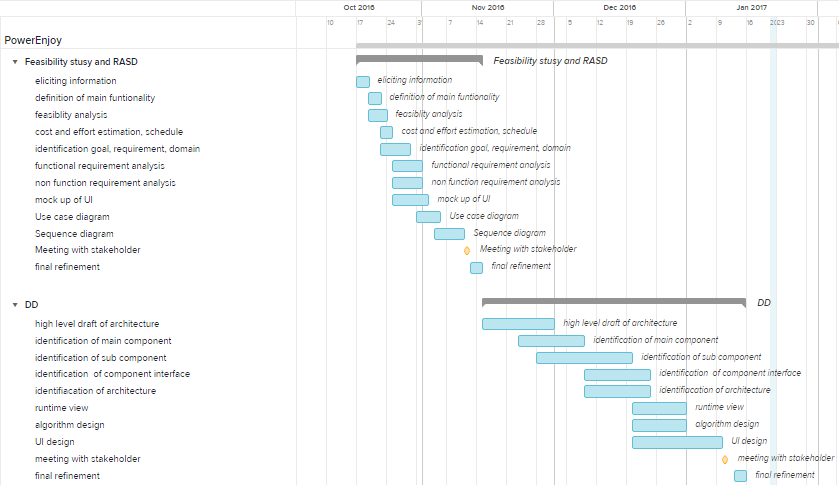
\includegraphics[width=1.2\textwidth]{schedule1.png} 
\end{figure}

\begin{figure}[H]
	\centering
	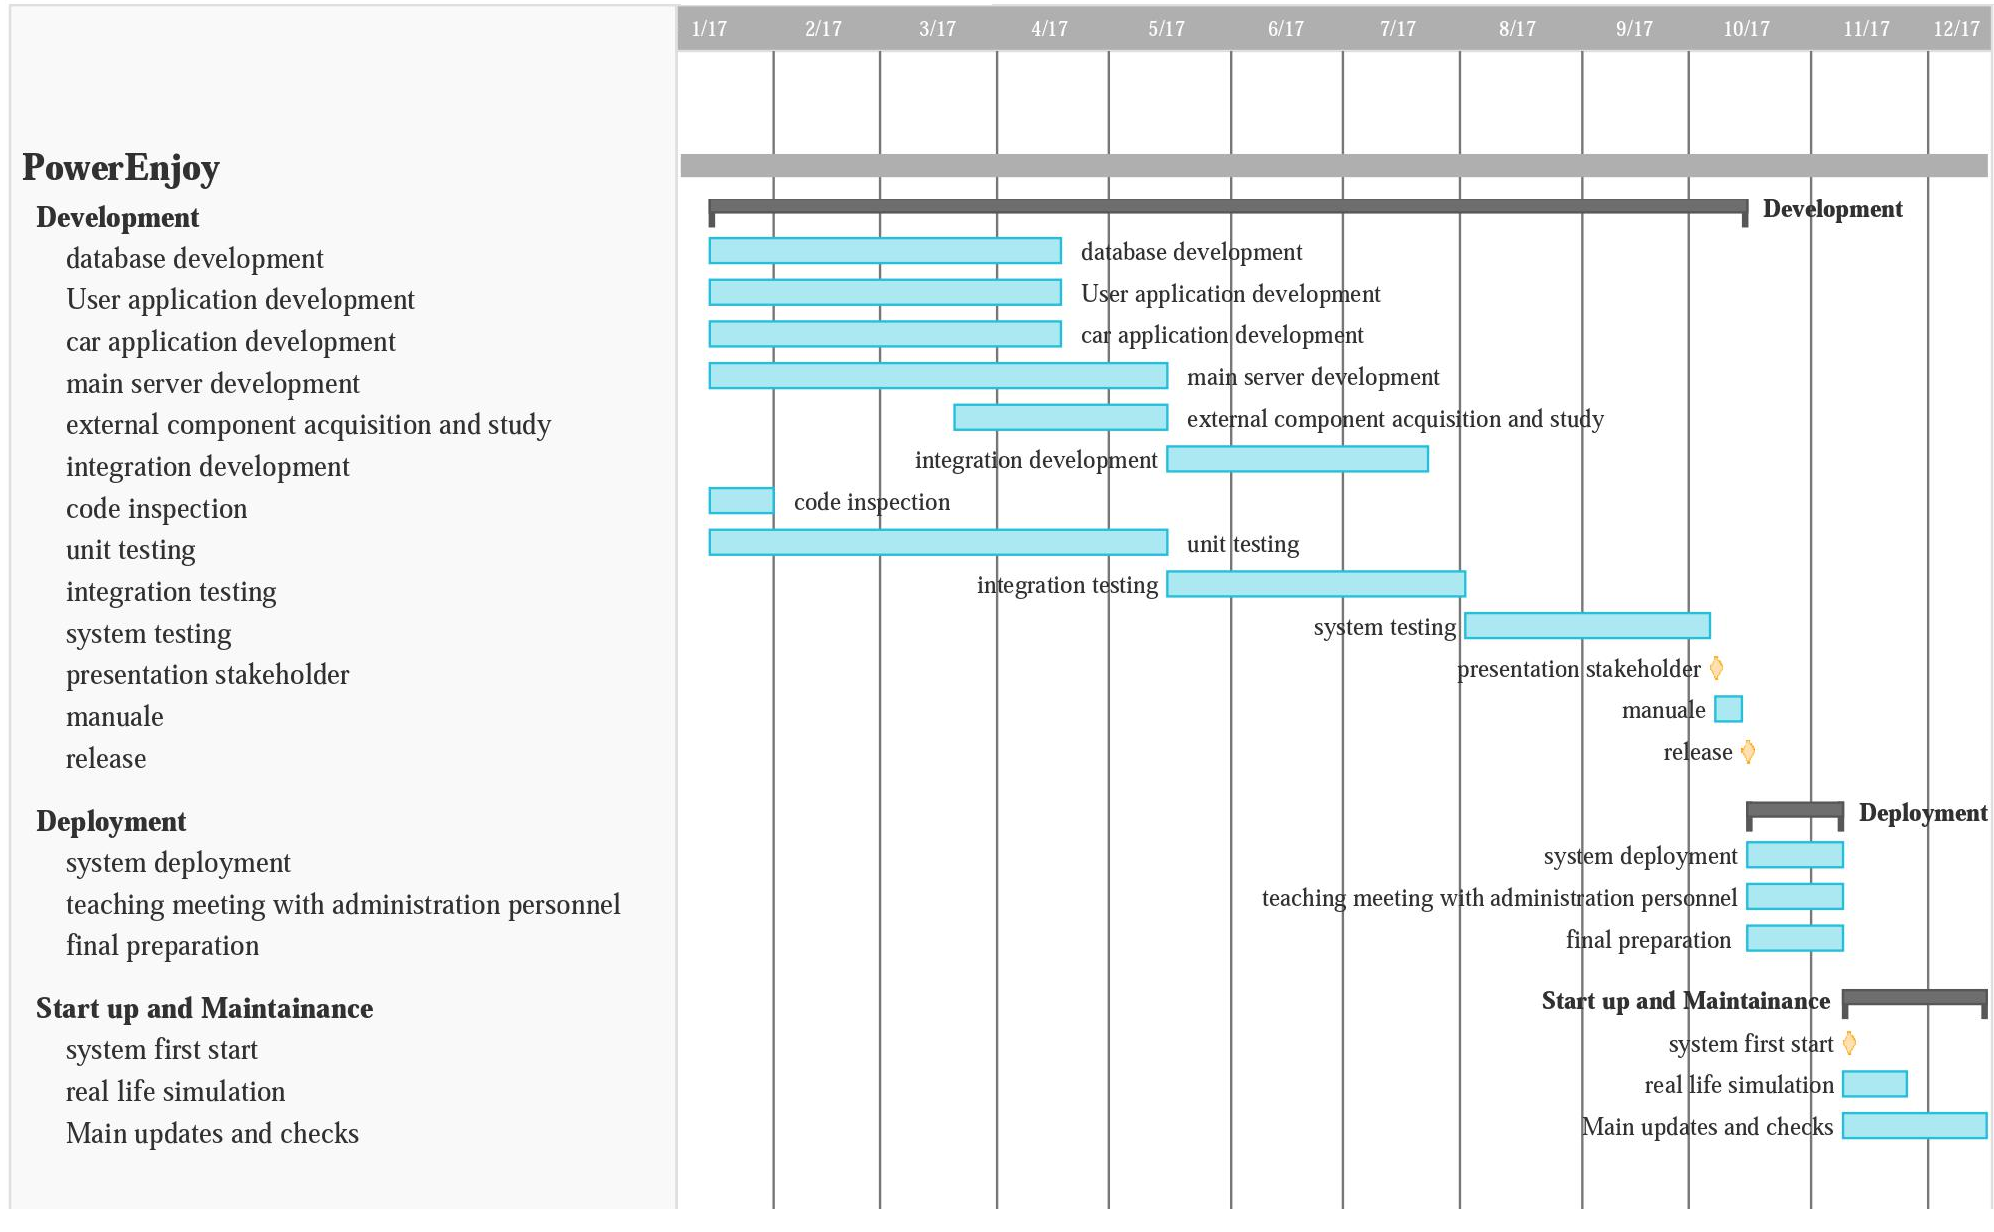
\includegraphics[width=1.2\textwidth]{schedule2.png} 
\end{figure}

\newpage
\section{Resource allocation}
In this chapter we going to continue the discourse of how to divide the work between development team. The table below shows the duration and the responsible member of each task.\\ \\Aforementioned person will organize detail human resource allocation of each job, aiming to guarantee the completeness within the deadline. So we will not provide the specific staff allocation chart.

\begin{figure}[H]
	\centering
	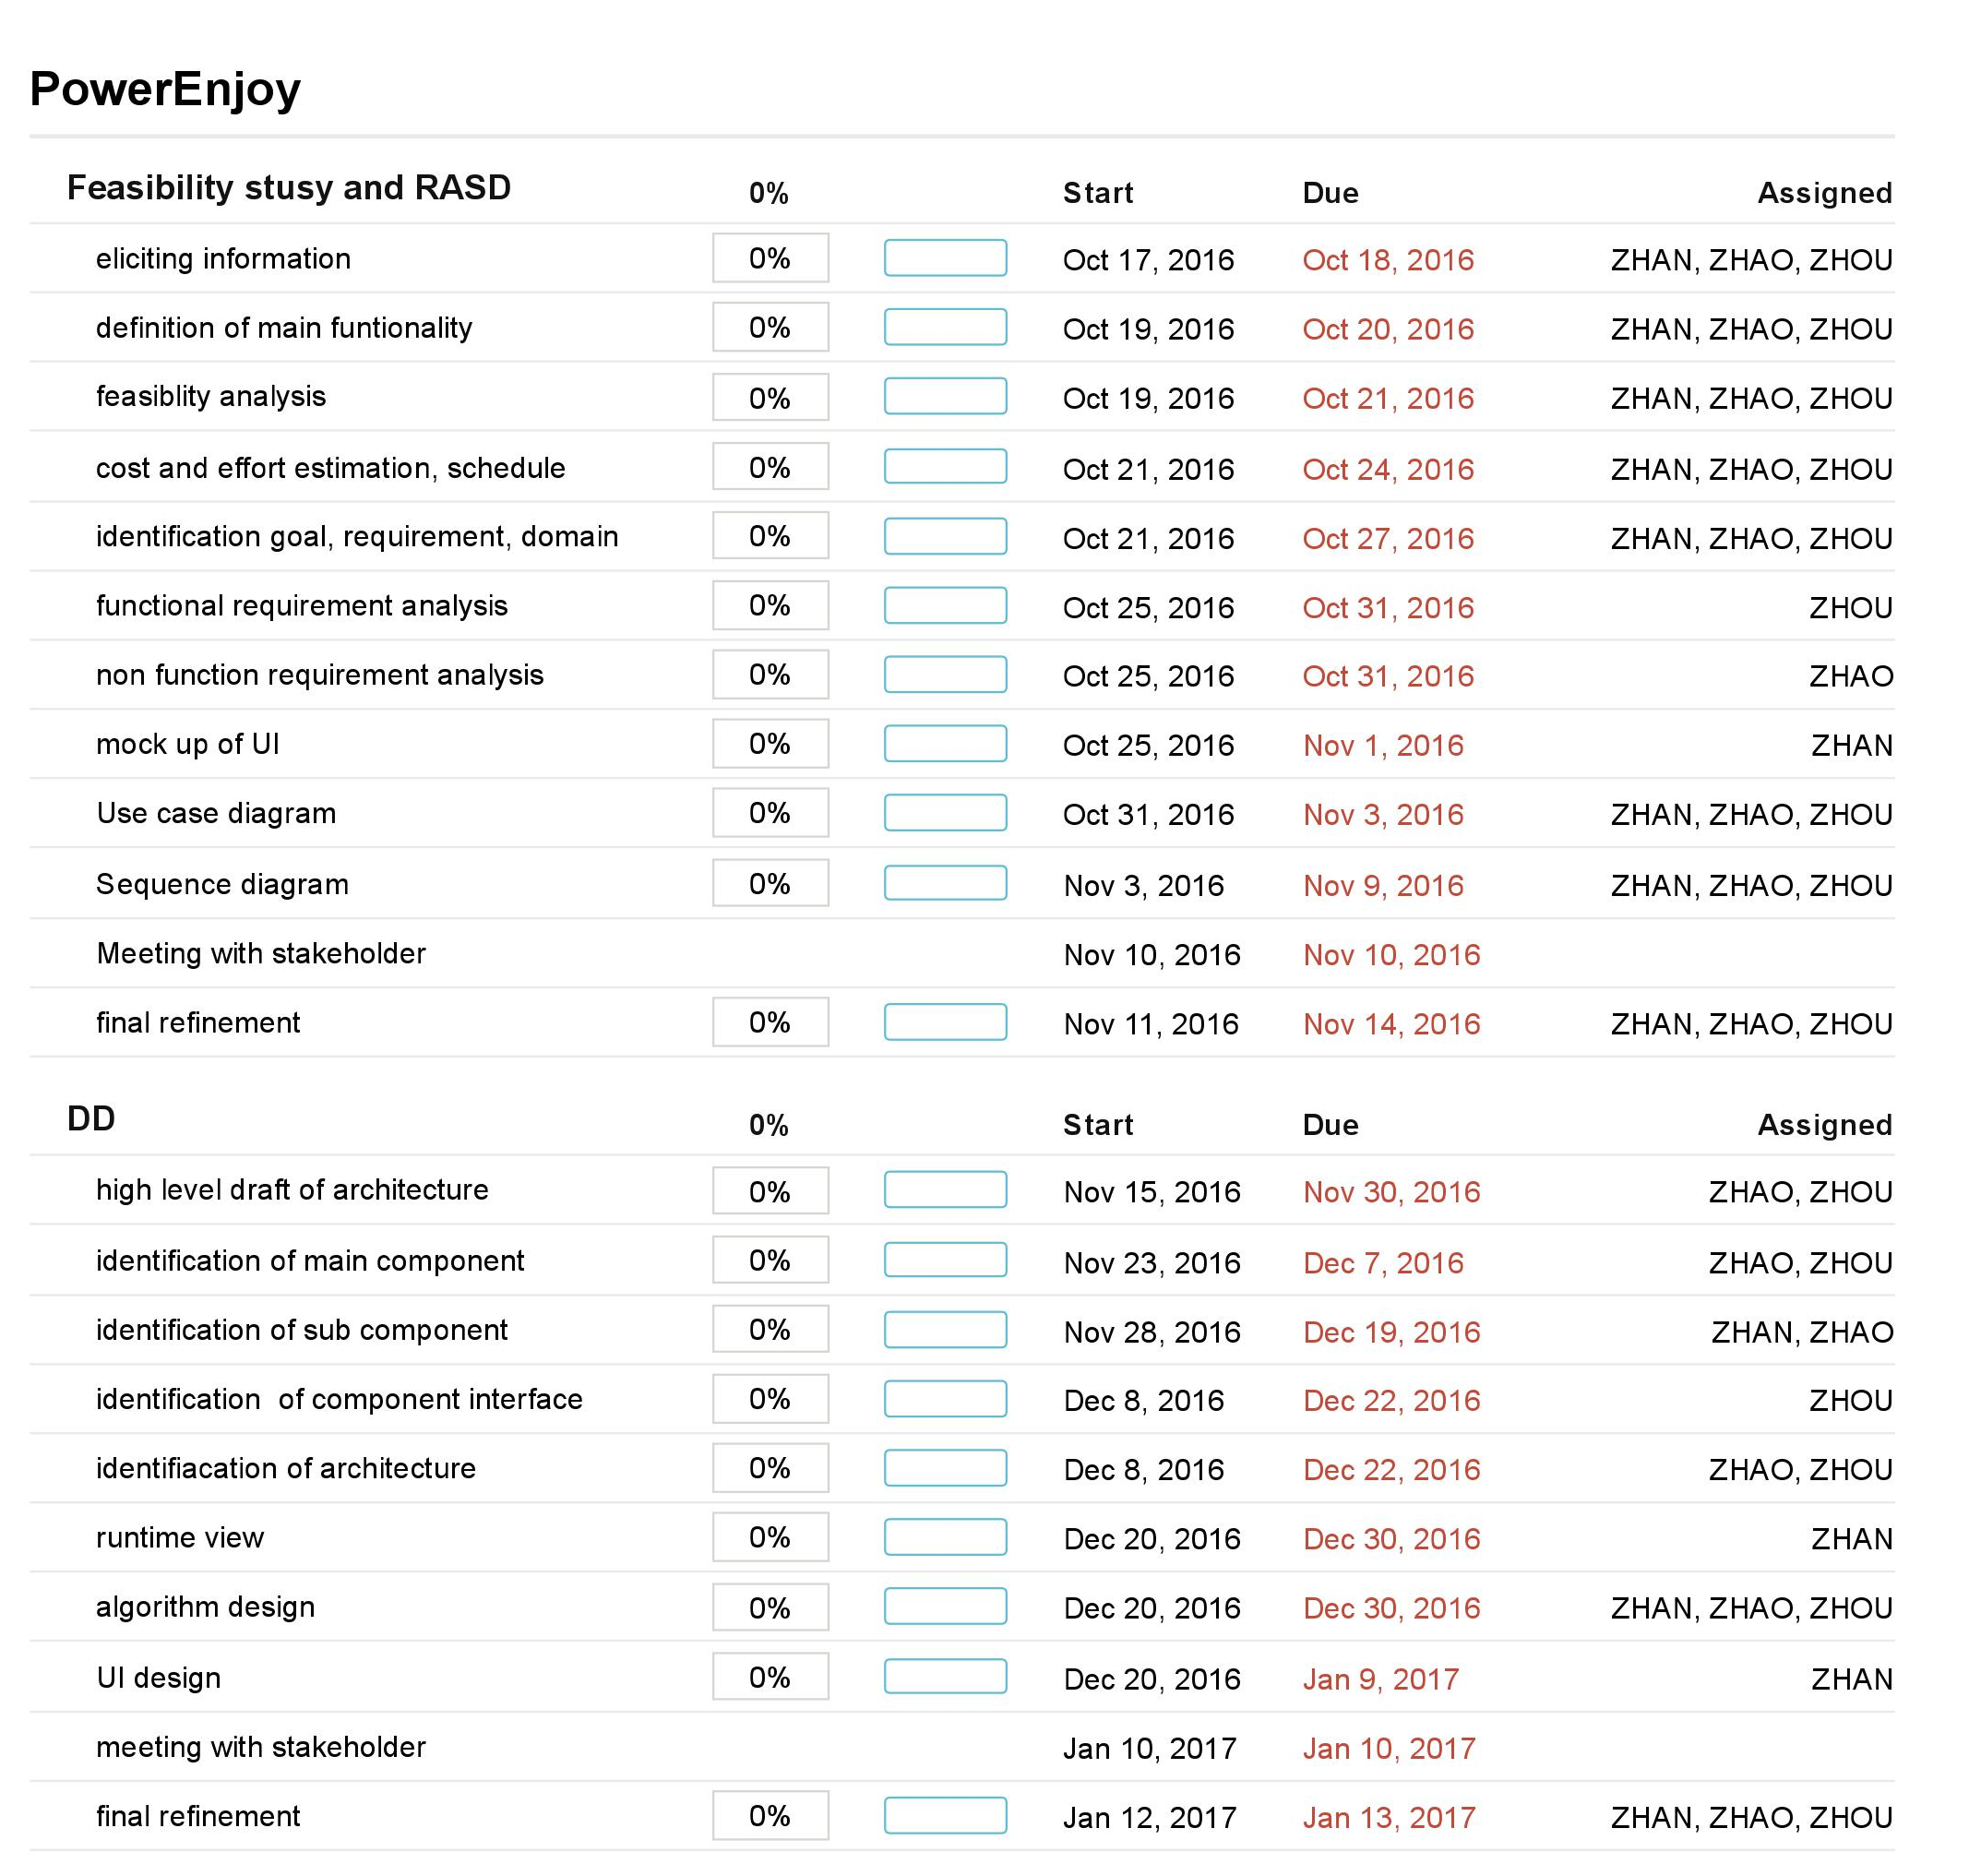
\includegraphics[width=\textwidth]{resource1.png} 
\end{figure}

\newpage
\begin{figure}[H]
	\centering
	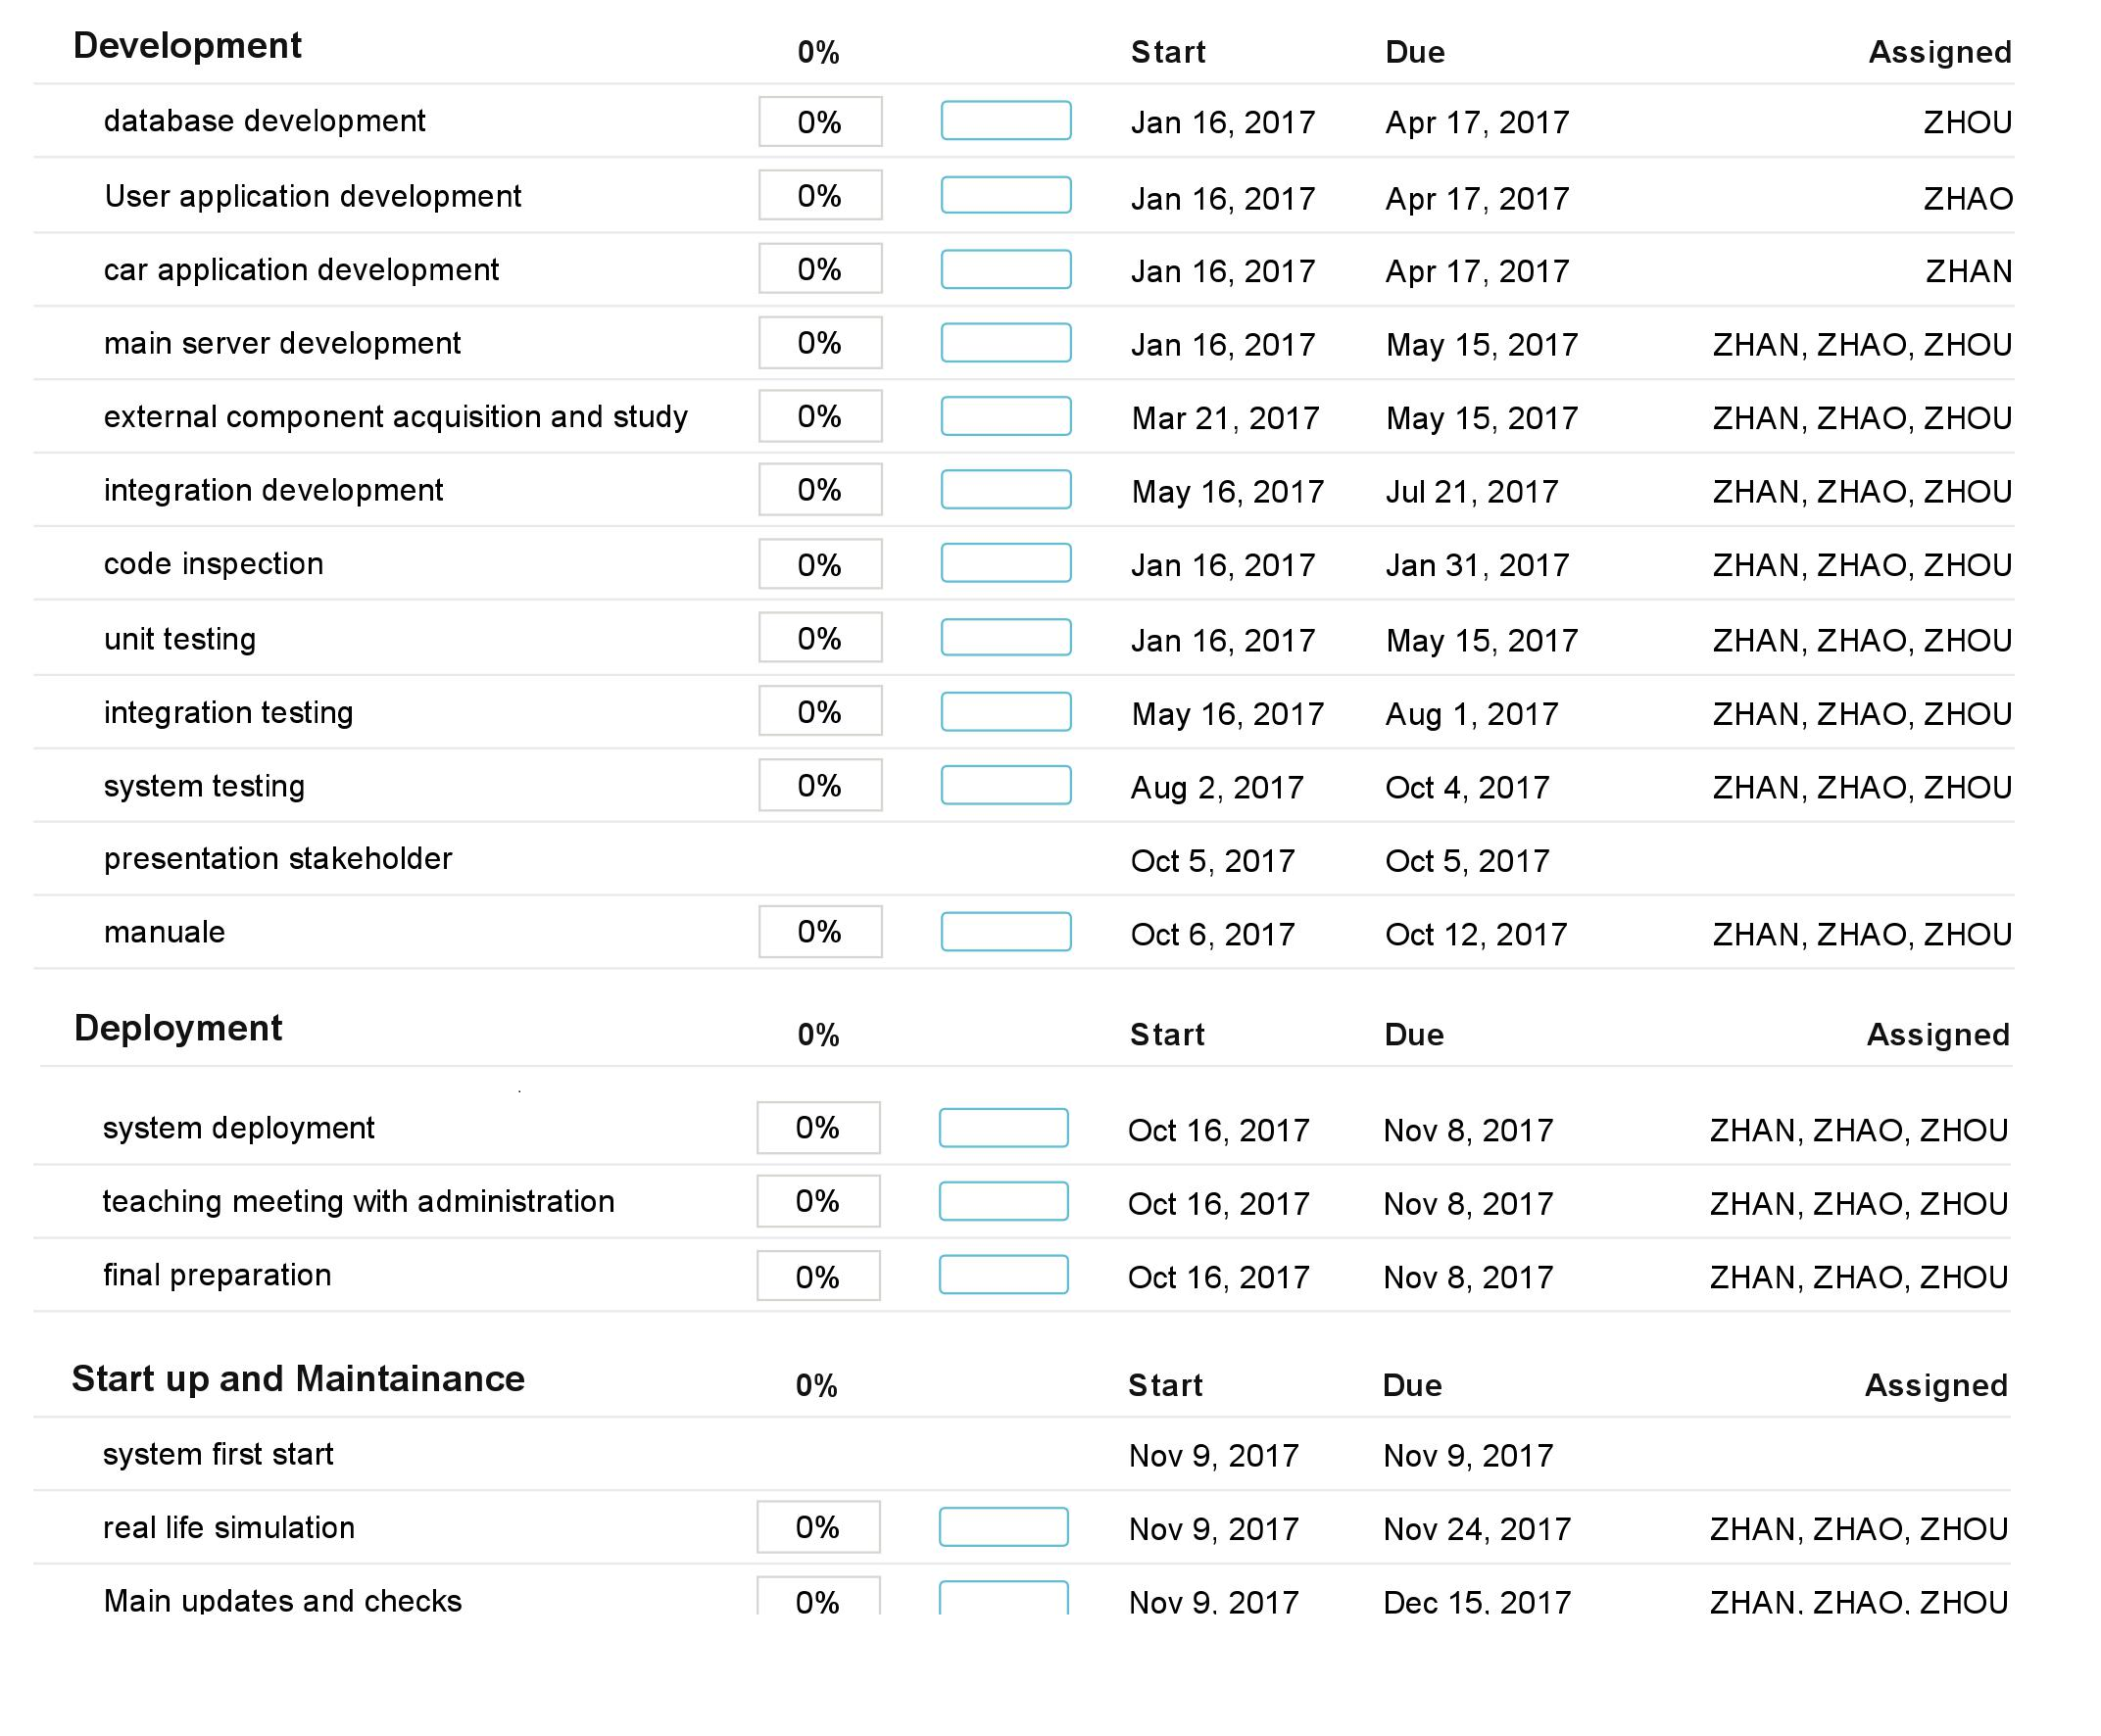
\includegraphics[width=\textwidth]{resource2.png}   
\end{figure}

\section{Risk management}
In this section, we'll analyze the risk we may encounter during the project development. Basically, there are three kinds of risks : Project risks, Technical risks, and Business risks. We'll present specific risks we may be trapped with and what we can do to deal with it. We use [L,M,H] to indicate the probability the risk will occur. [Low,Moderate,High]\\

The most possible risks come from the technical part. They threaten the quality and timeliness of the software to be produced. Some possible risks may be :
\begin{itemize}
	\item Wrong functionality [M]: Wrong functional quality can be a serious risk and lead to meaningless workload which increases the cost and slow down the project.\\
	To deal with wrong functionality, we adopt a proactive risk strategy. By better writing the RASD document and increase the meeting frequency with the stakeholders, we avoid this kind of risk. Also frequently report the project process and get feedback  from the stakeholders will help. 
	
	\item Wrong User Interface[M] : Wrong User Interface can lead to meaningless workload. \\
	To deal with it, we need to frequently meet with the stakeholders and make necessary discussion.
	
	\item Bad external components[L] : Bad external components are a major issue and threat to our project. Our project largely depend on the reliability of the following external components : Google Map, DBMS, Bank Service. In case any of them fail, we need to rewrite the business logic components and this leads to significant workload and time increase.
	
	Although the consequence is serious, the possibility of this risk to happen is actually low. Since the external components we choose to use is from huge and reliable companies like Google and Oracle. So we adopt a reactive risk strategy here. 
	
	\item Fail to accomplish logic components[L] : This risk is purely technical and there are no good solutions. Either we give programmers time to tick the task down or we recruit new employers with experience. Since the actual problem can be various, it is difficult to come up with a specific  prediction. Here we adopt a reactive strategy.
\end{itemize}

The project risk may arise during the software development. These risks mainly come from the stakeholder side.
\begin{itemize}
	\item Requirements volatility[M] : Requirement may change during the development. The point is we can not add too much constraints on our stakeholders. Here we adopt a proactive approach by organizing frequently meetings with the stakeholders. By doing this, we may avoid the risk and  minimize the negative consequence.
	\item Unrealistic schedule/budget[M] : This risk comes from both our own side and stakeholder side. During the development we may encounter various uncertain situations and risks which will slow down our process. Also budget may be tight. Here we adopt a reactive approach because we do not know how to come up with a efficient solution until we actually get trapped by the problem.
\end{itemize}
The third part of the risk is business risk. Some possible situations are presented below:
\begin{itemize}
	\item Management risk[L] : There is a possibility of losing the support of senior management due to a change in focus or a change in people. Since we assume there are three members in our development team, it is actually kind of critical issue, however the possibility is not high. So we adopt a reactive strategy here.
	\item Budget risk[L] : Losing budget or personnel commitment is not so likely in our case, so we adopt a reactive strategy here.
\end{itemize}


\newpage

\section{Effort}
\begin{itemize}
	\item 13/01/2017 ZHOU YINAN 2h document structure and introduction
	\item 14/012017	ZHOU YINAN 1h	Risk management
	\item 16/01/2017 ZHOU YINAN	2h Function points
	\item 16/01/2017 ZHAO KAIXIN 2h Scale Drivers
	\item 17/01/2017 ZHAO KAIXIN 5h Cost Drivers
	\item 18/01/2017 ZHAO KAIXIN 2h Effort Equations 
	\item 19/01/2017 ZHAN YUAN 5h Schedule graph
	\item 20/01/2017 ZHAN YUAN 1h Resource
\end{itemize}

\end{document}